\documentclass[openany]{book}

\usepackage[margin=1in]{geometry}
\usepackage{amsmath,amsfonts,amsthm, amssymb}
\usepackage{yhmath}
\usepackage{mathrsfs}
\usepackage{mathtools}
\usepackage{xcolor}
\usepackage{graphicx}
\usepackage{comment}
\usepackage{tikz-cd}
\usepackage{quiver}
\renewcommand{\familydefault}{ppl}
\newcommand{\tr}{\text{tr}}
\newcommand{\R}{\mathbb{R}}
\newcommand{\E}{\mathbb{E}}
\newcommand{\Z}{\mathbb{Z}}
\newcommand{\C}{\mathbb{C}}
\newcommand{\F}{\mathbb{F}}
\newcommand{\la}{\langle}
\newcommand{\ra}{\rangle}
\newcommand{\colim}{\text{colim}}
\DeclareMathOperator{\im}{im}
\let\oldemptyset\emptyset
\let\emptyset\varnothing
\newcommand{\tor}{\text{Tor}}
\newcommand{\id}{\text{id}}
\newcommand{\ext}{\text{Ext}}
\newcommand{\ptop}{\text{PTop}}
\newcommand{\pt}{\text{pt}}
\newcommand{\ach}{\text{Ach}}
\newcommand{\Q}{\mathbb{Q}}
\newcommand{\gal}{\text{Gal}}


\usepackage{thmtools,thm-restate}

% Fixing mdframed skip below
% See https://tex.stackexchange.com/a/292090/143086
\usepackage[framemethod=TikZ]{mdframed}
\usepackage{xpatch}
\makeatletter
\xpatchcmd{\endmdframed}
	{\aftergroup\endmdf@trivlist\color@endgroup}
	{\endmdf@trivlist\color@endgroup\@doendpe}
	{}{}
\makeatother

\definecolor{huilightpink}{HTML}{fcf2f9}
\definecolor{huidarkpink}{HTML}{ed34b3}
\declaretheoremstyle[
	mdframed={
		backgroundcolor=huilightpink,
		linecolor=huidarkpink,
		rightline=false,
		topline=false,
		bottomline=false,
		linewidth=2pt,
		innertopmargin=5pt,
		innerbottommargin=8pt,
		innerleftmargin=8pt,
		leftmargin=-2pt,
		skipbelow=2pt,
		nobreak
	},
	headfont=\normalfont\bfseries\color{huidarkpink}
]{huipinkbox}
\declaretheorem[style=huipinkbox,name=Theorem,within=chapter]{thm}
\declaretheorem[style=huipinkbox,name=Theorem,sibling=thm]{theorem}





\definecolor{huilightyellow}{HTML}{fff5d6}
\definecolor{huidarkyellow}{HTML}{fcad03}
\declaretheoremstyle[
	mdframed={
		backgroundcolor=huilightyellow,
		linecolor=huidarkyellow,
		rightline=false,
		topline=false,
		bottomline=false,
		linewidth=2pt,
		innertopmargin=5pt,
		innerbottommargin=8pt,
		innerleftmargin=8pt,
		leftmargin=-2pt,
		skipbelow=2pt,
		nobreak
	},
	headfont=\normalfont\bfseries\color{huidarkyellow}
]{huiyellowbox}
\declaretheorem[style=huiyellowbox,name=Proposition,within=chapter]{prop}

\definecolor{huilightpurple}{HTML}{faf2ff}
\definecolor{huidarkpurple}{HTML}{912ed9}
\declaretheoremstyle[
	mdframed={
		backgroundcolor=huilightpurple,
		linecolor=huidarkpurple,
		rightline=false,
		topline=false,
		bottomline=false,
		linewidth=2pt,
		innertopmargin=5pt,
		innerbottommargin=8pt,
		innerleftmargin=8pt,
		leftmargin=-2pt,
		skipbelow=2pt,
		nobreak
	},
	headfont=\normalfont\bfseries\color{huidarkpurple}
]{huipurplebox}
\declaretheorem[style=huipurplebox,name=Lemma,within=chapter]{lem}


\definecolor{huilightpurple}{HTML}{faf2ff}
\definecolor{huidarkpurple}{HTML}{912ed9}
\declaretheoremstyle[
	mdframed={
		backgroundcolor=huilightpurple,
		linecolor=huidarkpurple,
		rightline=false,
		topline=false,
		bottomline=false,
		linewidth=2pt,
		innertopmargin=5pt,
		innerbottommargin=8pt,
		innerleftmargin=8pt,
		leftmargin=-2pt,
		skipbelow=2pt,
		nobreak
	},
	headfont=\normalfont\bfseries\color{huidarkpurple}
]{huipurplebox}
\declaretheorem[style=huipurplebox,name=Definition,within=chapter]{defn}

\definecolor{huilightblue}{HTML}{edf9ff}
\definecolor{huidarkblue}{HTML}{4b79db}
\declaretheoremstyle[
	mdframed={
		backgroundcolor=huilightblue,
		linecolor=huidarkblue,
		rightline=false,
		topline=false,
		bottomline=false,
		linewidth=2pt,
		innertopmargin=5pt,
		innerbottommargin=8pt,
		innerleftmargin=8pt,
		leftmargin=-2pt,
		skipbelow=2pt,
		nobreak
	},
	headfont=\normalfont\bfseries\color{huidarkblue}
]{huiblueblox}
\declaretheorem[style=huiblueblox,name=Example,within=chapter]{example}

\declaretheoremstyle[
	mdframed={
		backgroundcolor=huilightblue,
		linecolor=huidarkblue,
		rightline=false,
		topline=false,
		bottomline=false,
		linewidth=2pt,
		innertopmargin=5pt,
		innerbottommargin=8pt,
		innerleftmargin=8pt,
		leftmargin=-2pt,
		skipbelow=2pt,
		nobreak
	},
	headfont=\normalfont\bfseries\color{huidarkblue}
]{huiblueblox}
\declaretheorem[style=huiblueblox,name=Problem,within=chapter]{prob}

\newcommand{\nirwarnsymbol}{%
	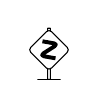
\begin{tikzpicture}[baseline=(x.base)]
		\draw[rounded corners=.01em] (-.05em,-1.07em)rectangle(.05em,.78em);
		\draw[fill=white,rounded corners=1.3] (0,.75em)--(.75em,0)--(0,-.75em)--(-.75em,0)--cycle;
		\draw[line width=0.2mm, line cap=round](-.4em,-1.07em)--(.4em,-1.07em);
		\node(x) at (0,0em) {};
		% Thank you https://tex.stackexchange.com/a/262510
		\draw[
			line cap=but,
			line join=round,
			x=.5em,
			line width=0.5mm,
			y=1*(height("Z")-\pgflinewidth)*(1-sin(10)),
			rotate=-10,
			rounded corners=1.5pt,
		](-0.57, 0.57) -- (0.57, 0.57) -- (-0.57, -0.57) -- (0.57, -0.57);
	\end{tikzpicture}%
}

%%%%%%%%%%%%%%%%%%%%%%%%%%%%%%%%%%%%%%%%%%%% MARGINS
\usepackage{marginnote}
% Thank you https://tex.stackexchange.com/a/472882
% Makes marginnotes always appear on the left, apparently
%
\makeatletter
\long\def\@mn@@@marginnote[#1]#2[#3]{%
	\begingroup
		\ifmmode\mn@strut\let\@tempa\mn@vadjust\else
			\if@inlabel\leavevmode\fi
			\ifhmode\mn@strut\let\@tempa\mn@vadjust\else\let\@tempa\mn@vlap\fi
		\fi
		\@tempa{%
			\vbox to\z@{%
				\vss
				\@mn@margintest
				\if@reversemargin\if@tempswa
						\@tempswafalse
					\else
						\@tempswatrue
				\fi\fi

					\llap{%
						\vbox to\z@{\kern\marginnotevadjust\kern #3
							\vbox to\z@{%
								\hsize\marginparwidth
								\linewidth\hsize
								\kern-\parskip
								%\mn@parboxrestore
								\marginfont\raggedleftmarginnote\strut\hspace{\z@}%
								\ignorespaces#1\endgraf
								\vss
							}%
							\vss
						}%
						\if@mn@verbose
							\PackageInfo{marginnote}{xpos seems to be \@mn@currxpos}%
						\fi
						\begingroup
							\ifx\@mn@currxpos\relax\else\ifx\@mn@currpos\@empty\else
									\kern\@mn@currxpos
							\fi\fi
							\ifx\@mn@currpage\relax
								\let\@mn@currpage\@ne
							\fi
							\if@twoside\ifodd\@mn@currpage\relax
									\kern-\oddsidemargin
								\else
									\kern-\evensidemargin
								\fi
							\else
								\kern-\oddsidemargin
							\fi
							\kern-1in
						\endgroup
						\kern\marginparsep
					}%
			}%
		}%
	\endgroup
}
\makeatother
%
% Mostly for todonotes
\renewcommand{\marginpar}{\marginnote}
%%%%%%%%%%%%%%%%%%%%%%%%%%%%%%%%%%%%%%%%%%%% /MARGINS

\definecolor{nirlightred}{RGB}{250, 220, 220}
\definecolor{nirdarkred}{HTML}{f40000}
\declaretheoremstyle[
	mdframed={
		backgroundcolor=nirlightred,
		linecolor=nirdarkred,
		rightline=false,
		topline=false,
		bottomline=false,
		linewidth=2pt,
		innertopmargin=5pt,
		innerbottommargin=8pt,
		innerleftmargin=8pt,
		leftmargin=-2pt,
		skipbelow=2pt,
		nobreak
	},
	headfont=\normalfont\bfseries\color{nirdarkred}
]{nirredbox}

% \makeatletter
% \declaretheorem[
% 	style=nirredbox,
% 	name=Warning,
% 	sibling=thm,
% 	% without \leavevmode, the first item in a list gets misformatted
% 	postheadhook={\leavevmode\marginnote{\nirwarnsymbol}[-3pt]%
% 	\ifthmt@thisistheone% restatable makes alignment weird
% 		\hspace{-2.2pt}%
% 	\fi}
% ]{warn}
% \makeatother

\newcommand{\nirideasymbol}{%
	
\begin{tikzpicture}[baseline=(x.base)]
		\draw[rounded corners=.01em] (-.05em,-1.07em)rectangle(.05em,.78em);
		\draw[fill=white,rounded corners=1.3] (0,.75em)--(.75em,0)--(0,-.75em)--(-.75em,0)--cycle;
		\draw[line width=0.2mm, line cap=round](-.4em,-1.07em)--(.4em,-1.07em);
		\node(x) at (0,0em) {};
		\node at (0,0em) {{\textbf{!}}};
	\end{tikzpicture}%
}
\renewcommand{\nirwarnsymbol}{%
	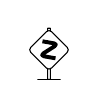
\begin{tikzpicture}[baseline=(x.base)]
		\draw[rounded corners=.01em] (-.05em,-1.07em)rectangle(.05em,.78em);
		\draw[fill=white,rounded corners=1.3] (0,.75em)--(.75em,0)--(0,-.75em)--(-.75em,0)--cycle;
		\draw[line width=0.2mm, line cap=round](-.4em,-1.07em)--(.4em,-1.07em);
		\node(x) at (0,0em) {};
		% Thank you https://tex.stackexchange.com/a/262510
		\draw[
			line cap=but,
			line join=round,
			x=.5em,
			line width=0.5mm,
			y=1*(height("Z")-\pgflinewidth)*(1-sin(10)),
			rotate=-10,
			rounded corners=1.5pt,
		](-0.57, 0.57) -- (0.57, 0.57) -- (-0.57, -0.57) -- (0.57, -0.57);
	\end{tikzpicture}%
}
\makeatletter
\declaretheorem[
	style=nirredbox,
	name=Idea,
	sibling=thm,
	% without \leavevmode, the first item in a list gets misformatted
	postheadhook={\leavevmode\marginnote{\nirideasymbol}[-3pt]%
	\ifthmt@thisistheone% restatable makes alignment weird
		\hspace{-2.2pt}%
	\fi}
]{idea}

\declaretheorem[
	style=nirredbox,
	name=Warning,
	sibling=thm,
	% without \leavevmode, the first item in a list gets misformatted
	postheadhook={\leavevmode\marginnote{\nirwarnsymbol}[-3pt]%
	\ifthmt@thisistheone% restatable makes alignment weird
		\hspace{-2.2pt}%
	\fi}
]{warn}
\makeatother

\title{Algebra Definition Theorem List}

\date{\today}
\author{Hui Sun}


\begin{document}

\maketitle

\tableofcontents
\newpage

\chapter{Group Theory I}
This corresponds to Aluffi Chapter II.

\begin{prop}
    Let $G$ be a group, for all $a,g,h\in G$, if 
    \begin{equation*}
        ga=ha
    \end{equation*}
    then $g=h$.
\end{prop}

\begin{prop}
    Let $g\in G$ have order $n$, then 
    \begin{equation*}
        n\mid |G|
    \end{equation*}
\end{prop}

\begin{cor}
    If $g$ is an element of finite order, and let $N\in\mathbb{Z}$, then 
    \begin{equation*}
        g^N=e \iff N \text{ is a multiple of }|g|
    \end{equation*}
\end{cor}

\begin{prop}
    Let $g\in G$ be of finite order, then $g^m$ also has finite order, for all $m\geq 0$, and 
    \begin{equation*}
        \left|g^m\right|=\frac{\text{lcm}(m,|g|)}{m}=\frac{|g|}{\gcd(m,|g|)}
    \end{equation*}
\end{prop}

\begin{prop}
    If $gh=hg$, then $|gh|$ divides $\text{lcm}(|g|,|h|)$.
\end{prop}


\begin{defn}[Dihedral Group]
    Let $D_{2n}$ denote the group of symmetries of a $n$-sided polynomial, consisting of $n$ rotations and $n$ reflections about lines trhough the origin and a vertex or a midpoint of a side.
\end{defn}

\begin{prop}
    Let $m\in\Z/n\Z$, then 
    \begin{equation*}
        |m|=\frac{n}{\gcd(n,m)}
    \end{equation*} 
\end{prop}

\begin{cor}
    The element $m\in\Z/n\Z$ generates $\Z/n\Z$ if and only if $\gcd(m,n)=1$.
\end{cor}


\begin{defn}[Multiplicative $(\Z/n\Z)^\times$]
    The multiplicative group of $\Z/n\Z$ is 
    \begin{equation*}
        \left(\Z/n\Z\right)^\times=\left\{m\in\Z/n\Z: \gcd(m,n)=1\right\}
    \end{equation*}
\end{defn}

\begin{prop}
    Let $\varphi:G\to H$ be a homomorphism, and let $g\in G$ be an element of finite order, then $|\varphi(g)|$ divides $|g|$.

    For example, there is no nontrivial homomorphism from $\Z/n\Z$ to $\Z$.
\end{prop}

\begin{prop}
    There is an isomorphism between $D_6$ and $S_3$.
\end{prop}

\begin{prop}
    Let $\varphi: G\to H$ be an isomorphism, for all $g\in G$, $|\varphi(g)|=|g|$, and $G$ is commutative if and only if $H$ is commutative.
\end{prop}

\begin{prop}
    If $H$ is commutative, then $\text{Hom}(G,H) $ is a group.
\end{prop}

\begin{defn}
    Let $A=\{1,\dots, n\}$, then the free abeliean group on $A$ is 
    \begin{equation*}
        \Z\oplus\dots\oplus\Z=\Z^{\oplus n}
    \end{equation*}
\end{defn}
\begin{prop}
    For every set $A$, the free abelian group $A$ is 
    \begin{equation*}
        \Z^{\oplus A}
    \end{equation*}
    In other words, any element in the free abelian group of $A$ can be written as 
    \begin{equation*}
        \sum_{a\in A}m_aj(a)
    \end{equation*}
    where $m_a\neq 0$ for only finitely many terms, and 
    \begin{equation*}
        j_a(m)=\begin{cases}
            1, m=a\\
            0, m\neq a
        \end{cases}
    \end{equation*}
\end{prop}

\begin{prop}
    Let $\{H_\alpha\}$ be any family of subgroups of $G$, then 
    \begin{equation*}
        \bigcap_\alpha H_\alpha
    \end{equation*}
    is a subgroup of $G$.
\end{prop}

\begin{prop}
    If $\varphi: G_1\to G_2$ is a group homomorphism, then if $H_2\subset G_2$ is a subgroup, then 
    \begin{equation*}
        \varphi^{-1}(H_2)
    \end{equation*}
    is a subgroup of $G_1$.
\end{prop}

\begin{prop}
    Let $H\subset\Z/n\Z$ be a subgroup, then $H$ is generated by some $m$ where $m$ divides $n$.
\end{prop}


\begin{prop}
    If $\varphi: G_1\to G_2$ is a homomorphism, then $\ker(\varphi)$ is a normal subgroup.
\end{prop}


\begin{thm}
    Let $\varphi:G_1\to G_2$ be a surjective homomorphism, then 
    \begin{equation*}
        G_2=\frac{G_1}{\ker\varphi}
    \end{equation*}
\end{thm}

\begin{prop}
    Let $H_1,H_2$ be normal subgroups of $G_1,G_2$, then $H_1\times H_2$ are normal subgroups of $G_1\times G_2$, then 
    \begin{equation*}
        \frac{G_1\times G_2}{H_1\times H_1}\cong\frac{G_1}{H_1}\times\frac{G_2}{H_2}
    \end{equation*}

    For example, 
    \begin{equation*}
        \frac{S_3}{\Z/3\Z}=\frac{\Z}{2\Z}
    \end{equation*}
\end{prop}

\begin{prop}
    Let $H$ be a normal subgroup of $G$, then every subgroup containing $H$ can be identified with a subgroup $K/H$ of $G/H$.
\end{prop}


\begin{prop}
    Let $H$ be a normal subgroup of $G$, and $N$ be a subgroup of $G$ containing $H$, then $N/H$ is normal in $G/H$ if and only if $N$ is normal in $G$, in this case
    \begin{equation*}
        \frac{G/H}{N/H}=\frac{G}{N}
    \end{equation*}
\end{prop}



\begin{prop}
    Let $H,K$ be subgroups of $G$, and if $H$ is normal, then $HK$ is a subgroup of $G$ and $H$ is normal in $HK$. Moreover, $H\cap K$ is normal in $K$, and 
    \begin{equation*}
        \frac{HK}{H}\cong\frac{K}{H\cap K}
    \end{equation*}
\end{prop}


\begin{prop}
    Let $H$ be a subgroup of $G$, then for all $g\in G$, the function 
    \begin{equation*}
        H\to gH, h\mapsto gh
    \end{equation*}
    is a bijection.
\end{prop}

\begin{thm}[Lagrange]
    If $G$ is a fintie group, and $H\subset G$ is a subgroup, then 
    \begin{equation*}
        |G|=[G:H]\cdot|H|
    \end{equation*}
    In particular, $|H|$ divides $|G|$.
\end{thm}

\begin{thm}[Fermat's Little Theorem]
    Let $p$ be a prime integer, and $a$ be any integer, then 
    \begin{equation*}
        a^p\equiv a\mod p
    \end{equation*}
\end{thm}

% \begin{defn}[action]
%     An action of a group $G$ on a set $A$ is a homomorphism $\varphi: G\to \text{Aut}(A)$, 
% \end{defn}

\begin{prop}
    Any group $G$ acts on itself by left/right multiplications, and acts on the costs $G/H$:
    \begin{equation*}
        \varphi: g\mapsto \left(aH\mapsto gaH\right)
    \end{equation*}
\end{prop}


\begin{defn}[orbit]
    The orbit of $a\in A$ of a group action by $G$ is 
    \begin{equation*}
        O(a)=\left\{g\cdot a: g\in G\right\}
    \end{equation*}
    The stabilizer of $a$ is the following 
    \begin{equation*}
        \text{Stab}_G(a)=\left\{g\in G: g\cdot a=a\right\}
    \end{equation*}
\end{defn}

\begin{prop}
    The orbits of an action form a partition on the set $A$, and $G$ acts transitively on each orbit.
\end{prop}

\begin{defn}[transitive action, faithful action]




    An action of $G$ on $A$ is transitive if for all $a,b\in G$, there exists $g\in G$ such that 
    \begin{equation*}
        g\cdot a=b
    \end{equation*}
    In other words, the orbit of any element $a\in A$ is the entire set.

    An action is faithful if for any $g\in G$, 
    \begin{equation*}
        g\cdot a=a \text{ for all } a
    \end{equation*}
    implies that $g=e$.
\end{defn}



\begin{prop}
    Every transitive action of $G$ on a set $A$ is isomorphic to multiplication of $G$ on $G/H$, where $H=\text{Stab}(a)$ for any $a\in A$.
\end{prop}


\begin{prop}
    If $O(a)$ is an orbit of the action of a finite group $G$, then $O(a)$ is a finite and $|O|$ divides $|G|$. Moreover, 
    \begin{equation*}
        |G|=|O(a)|\cdot|\text{Stab}_G(a)|
    \end{equation*}

    For example,there is no transitive action of $S_3$ on the set of $5$ elements. 
\end{prop}











\chapter{Group Theory II}
This corresponds to Aluffi Chapter IV.

\begin{prop}[class formula]
    Let $S$ be a finite set, and $G$ act on $S$, then 
    \begin{equation*}
        |S|=|Z|+\sum_{a\in A}[G: \text{Stab}(a)]=|Z|+\sum_{a\in A}|O_a|
    \end{equation*} 
    where $Z=\left\{a\in S: g\cdot a=a\text{ for all } g\right\}$, i.e., the fixed elements, and $A\subset S$ contains exactly one element from each nontrivial orbit of the action. 
    
    In other words, $|S|$ is the sum of the number of trivial orbits and each nontrivial orbit.
\end{prop}

\begin{prop}
    Let $G$ be a $p$-group that acts on a finite set $S$, then let $Z$ be fixed elements of this acion, then 
    \begin{equation*}
        |S|\equiv |Z|\mod p
    \end{equation*}
\end{prop}


\begin{prop}
    Let $G$ be finite, and if $G/Z(G)$ is cyclic, then $G$ is abelian.
\end{prop}

\begin{defn}[centralizer, conjugacy class]
    The centralizer $Z_G(g)$ where $g\in G$ is its stabilizer under conjugation:
    \begin{equation*}
        Z_G(g)=\left\{h\in G: hgh^{-1}=g\right\}
    \end{equation*}
    The conjugacy class of $g\in G$ is the orbit $[g]$ of the conjugation action.
\end{defn}


\begin{prop}[Class formula]
    Let $G$ be finite, then 
    \begin{equation*}
        |G|=|Z(G)|+\sum_{a\in A}[a]
    \end{equation*}
    where $A$ contains one representative for each nontrivial conjugacy class.
\end{prop}


\begin{cor}
    Let $G$ be a nontrivial $p$-group, then $G$ has a nontrivial center.
\end{cor}

\begin{prop}
    The only possibility for the class formula of a nonabelian group of order $6$ is 
    \begin{equation*}
        6=1+2+3
    \end{equation*}
    The center must be trivial if $G$ is nonabelian.
\end{prop}


\begin{defn}[normalizer]
    Let $A\subset G$ be a subset. The normalizer $N_G(A)$ of $A$ is 
    \begin{equation*}
        \text{Stab}_G(A)=\left\{g: gAg^{-1}=A\right\}
    \end{equation*}
    The centralizer of $A$ is the subgroup $Z_G(A)\subset N_G(A)$ fixing each $a\in A$:
    \begin{equation*}
        Z_G(A)=\left\{ g: gag^{-1}=a \text{ for all } a\in A\right\}
    \end{equation*}

    If $H$ is subgroup of $G$, every conjugate $gHg^{-1}$ is also a subgroup of $G$, and all conjugate groups have the same order.
\end{defn}

\begin{prop}
    $H$ is a normal subgroup of $G$ if and only if $N_G(H)=G$. More generally, the normalizer $N_G(H)$ for any subgroup $H$ is the largest subgroup of $G$ in which $H$ is normal.
\end{prop}

\begin{prop}
    Let $H\subset G$ be a subgroup, then the number of subgroups conjugate to $H$ is equal to $[G:N_G(H)]$.
\end{prop}
\begin{cor}
    If $[G:H]$ is finite, then the number of subgroups conjugate to $H$ is finite, and 
    \begin{equation*}
        [G:H]=[G:N_G(H)]\cdot[N_G(H): H]
    \end{equation*}
    In other words, the number of subgroups conjugate to $H$ divides the index $[G:H]$.
\end{cor}


\begin{thm}[Cauchy's Theorem]
    Let $G$ be a finite group, and let $p$ be a prime divisor of $|G|$, then $G$ contains an element of order $p$.

    Moreover, let $N$ be the number of cyclic subgroups of order $p$, then 
    \begin{equation*}
        N\equiv 1\mod p
    \end{equation*}
\end{thm}


\begin{defn}[simple]
    A group is simple if it is nontrivial and its only normal subgroups are $\{e\}$ and $G$ (has no nontrivial proper subgroup).
\end{defn}

\begin{defn}[$p$-Sylow subgroups]
    Let $p$ be prime, a $p$-Sylow subgroup of a finite group $G$ is a subgroup of order $p^r$, where $|G|=p^rm$, $\gcd(p,m)=1$. 
\end{defn}

\begin{thm}[Sylow I]
    Every finite group contains a $p$-Sylow subgroup for all prime $p$. If $p^k$ divides $|G|$, then $G$ has a subgroup of order $p^k$.
\end{thm}

\begin{thm}[Sylow II]
    Let $G$ be finite, and $P$ is a $p$-Sylow subgroup, let $H\subset G$ be a $p$-group, then $H$ is contained in a conjugate of $P$. If $P_1,P_2$ are both $p$-Sylow subgroups, then they are conjugates to each other.
\end{thm}

\begin{thm}[Sylow III]
    Let $|G|=p^rm$, and $\gcd(p,m)=1$, then the number of $p$-Sylow subgroups is 
    \begin{equation*}
        n_p\mid m 
    \end{equation*}
    and 
    \begin{equation*}
        n_p\equiv 1\mod p
    \end{equation*}
\end{thm}

\begin{prop}
    Let $G$ be a group of order $mp^r$, where $p$ is prime and $1<m<p$, then $G$ is not simple.
\end{prop}


\begin{prop}
    Let $p<q$ be primes, let $G$ has order $pq$, if $p\nmid (q-1)$, then $G$ is cyclic.
\end{prop}

\begin{prop}
    Let $q$ be an odd prime, and $G$ be a noncommutative group of order $2q$, then 
    \begin{equation*}
        G\cong D_{2q}
    \end{equation*}
\end{prop}


\begin{defn}[commutator subgroup]
    Let $G$ be a group, the commutator subgroup of $G$ is the subgroup \textbf{generated} by all elements 
    \begin{equation*}
        ghg^{-1}h^{-1}
    \end{equation*}
\end{defn}


\begin{prop}
    Let $[G,G]$ be the commutator subgroup of $G$, then $[G,G]$ is normal in $G$, and the quotient, also called the abelianization of $G$, 
    \begin{equation*}
        G^{\text{ab}}=\frac{G}{[G,G]}
    \end{equation*}
    is commutative.

    If $\varphi: G\to H$, where $H$ is commutative, then 
    \begin{equation*}
        [G,G]\subset\ker(\varphi)
    \end{equation*}
\end{prop}
\begin{defn}
    A group $G$ is solvable, if ther exists a sequence such that 
    \begin{equation*}
        \{e\}=G_0\subset\dots\subset G_k=G
    \end{equation*}
    where $G_i$ is normal in $G_{i+1}$, and $G_{i+1}/G_i$ is abelian, or equivalently, cyclic.
\end{defn}


\begin{prop}
    All $p$-groups are solvable!
\end{prop}

\begin{prop}
    Let $N$ be normal in $G$, then $G$ is solvable if and only if $N, G/N$ are solvable.
\end{prop}

\begin{prop}
    Disjoint cycles commute. For every $\sigma\in S_n$, $\sigma$ can be written as disjoint nontrivial cycles, unique up to rearranging.
\end{prop}

\begin{prop}
    Two elements in $S_n$ are conjugate in $S_n$ if and only if they have the same type. Hence the number of conjugacy classes is the number of partitions of $n$ as a sum.
\end{prop}

\begin{prop}
    Normal subgroups are unions of conjugacy classes. 

    One can use this fact to show that there is no normal subgroup of order 30 in $S_5$. 
\end{prop}

\begin{defn}[Even permutation]
    Let $\sigma\in S_n$, then $\sigma$ is even if 
    \begin{equation*}
        \prod_{i<j}(x_{\sigma(i)}-\sigma(j))=\prod_{i<j}(x_i-x_j)
    \end{equation*}
\end{defn}

\begin{defn}
    The alternating group $A_n$ consists of even permutations of $\sigma\in S_n$, and 
    \begin{equation*}
        [S_n:A_n]=2
    \end{equation*}
\end{defn}


\begin{prop}
    Let $\sigma\in A_n$, where $n\geq 2$, then the conjugacy class of $\sigma$ in $S_n$ splits into two conjugacy classes in $A_n$ precisely if the type of $\sigma$ consists of distinct odd numbers. 

    For example, the $5$-cycle of $S_5$ splits into $2$ conjugacy classes in $A_5$.
\end{prop}

\begin{prop}
    The group $A_5$ is a simple noncommutative group of order $60$ 
\end{prop}
\begin{proof}
    Any nontrivial normal subgroup consists of nontrivial conjugacy classes and $\{e\}$, the conjugacy classes of $A_5$ has the following size:
    \begin{equation*}
        1, 15, 20, 12, 12
    \end{equation*}
    Thus any subgroup of $G$, i.e., order that divides $60$ cannot be written as a sum of the numbers above.
\end{proof}

\begin{prop}
    The alternating group is generated by $3$-cycles.
\end{prop}

\begin{prop}
    Let $n\geq 5$, if a normal subgroup of $A_n$ contains a $3$-cycle, then it contaisn all $3$-cycles.
\end{prop}
\begin{proof}
    It suffices to note that the $3$ cycles form a conjugacy class that doesn't split from $S_n$ to $A_n$.
\end{proof}
\begin{thm}
    The alternating group is simple for $n\geq 5$.

    As a corollary, $S_n$ is not solvable for $n\geq 5$.
\end{thm}


\begin{prop}
    Let $N,H$ be normal subgroups of $G$, then 
    \begin{equation*}
        [N,H]\subset N\cap H
    \end{equation*}
    where $[N,H]$ is the commutator of $N,H$.
\end{prop}

\begin{prop}
    Let $N,H$ be normal subgroups, and $N\cap H=\{e\}$, then $N,H$ commute with each other.
\end{prop}

\begin{thm}
    Let $N,H$ be normal subgroups of $G$, such that $N\cap H=\{e\}$, then 
    \begin{equation*}
        NH\cong N\times H
    \end{equation*}
\end{thm}


\begin{defn}[Short exact sequence]
    A short exact sequence of groups is a sequence:
    \[\begin{tikzcd}
        1 & N & G & H & 1
        \arrow[from=1-1, to=1-2]
        \arrow["\varphi", from=1-2, to=1-3]
        \arrow["\psi", from=1-3, to=1-4]
        \arrow[from=1-4, to=1-5]
    \end{tikzcd}\]
    where $\psi$ surjective and $\varphi$ is injective, and $N$ is normal in $\varphi$ which induces an isomorphism $G/N\cong H$.

    A SES splits if $H$ is identified with a subgroup of $G$ such that 
    \begin{equation*}
        N\cap H=\{e\}
    \end{equation*}
\end{defn}


\begin{defn}[semidirect product]
    Let $N$ be a normal subgroup, and let $\theta: H\to\text{Aut}(N)$, then define an operator $\cdot_\theta$ as 
    \begin{equation*}
        (n_1,h_1)\cdot_\theta(n_2,h_2)=(n_1\theta(h_1)(n_2), h_1h_2)
    \end{equation*}
    The semidirect product of $N\rtimes_\theta$ is the group $N\times H$ with operator $\cdot_\theta$.
\end{defn}

\begin{thm}
    Let $N,H$ be groups, and $\theta: H\to\text{Aut}(N)$, let $G=N\rtimes_\theta H$, then 
    \begin{enumerate}
        \item $G$ contains isomorphic copies of $N,H$.
        \item The natural projection $G\to H$ is surjective, with kernel $N$, thus $N$ is normal in $G$ and the sequence 
        \[\begin{tikzcd}
            1 & N & {N\rtimes_\theta H} & H & 1
            \arrow[from=1-1, to=1-2]
            \arrow[from=1-2, to=1-3]
            \arrow[from=1-3, to=1-4]
            \arrow[from=1-4, to=1-5]
        \end{tikzcd}\]
        is split exact.
        \item $N\cap H=\{e\}$.
        \item $G=NH$.
        \item The homomorphism is conjugation: 
        \begin{equation*}
            \theta(h)(n)=hnh^{-1}
        \end{equation*}
    \end{enumerate}
\end{thm}

\begin{prop}
    Let $N,H$ be subgroups, and $N$ is normal, suppose that $N\cap H=\{e\}$, and $G=NH$, then let $\theta: H\to\text{Aut}(N)$ be 
    \begin{equation*}
        \theta(h)n=nhn^{-1}
    \end{equation*}
    Then 
    \begin{equation*}
        G\cong N\rtimes_\theta H
    \end{equation*}
\end{prop}


\begin{prop}
    Let $G$ be abelian, let $H,K$ be subgroups such that $|H|, |N|$ are relatively prime, then 
    \begin{equation*}
        H+K\cong H\oplus K
    \end{equation*}
\end{prop}
\begin{proof}
    Lagrange.
\end{proof}
\begin{prop}
    Every finite abelian group is a direct sum of its nontrivial Sylow subgroups.
\end{prop}


\begin{prop}
    Let $p$ be prime, and $r\geq 1$, let $G$ be a noncyclic abelian group of order $p^{r+1}$, then let $g\in G$ be an element of order $p^r$, then there exists an element $h\in G$ such that $h\not\in\la g\ra$, such that $|h|=p$.

    If $G$ is finite and abelian, then $G$ is a direct sum of cyclic groups, which may be assumed to be cyclic $p$-groups.
\end{prop}



\begin{thm}
    Let $G$ be finite nontrivial abelian group, then there exists prime integers $p_1,\dots, p_r$, and positive integers $n_{i(j)}$ such that 
    \begin{equation*}
        G=\bigoplus_{i,j}\frac{\Z}{p_i^{n_{i(j)}}\Z}
    \end{equation*}
    There exists positive integers $1<d_1\mid \dots\mid d_s$ such that $|G|=d_1\dots d_s$, and 
    \begin{equation*}
        G\cong\frac{\Z}{d_1\Z}\oplus\dots\oplus\frac{\Z}{d_s\Z}
    \end{equation*}
\end{thm}



\begin{thm}
    Let $F$ be a field, and $G$ be a finite subgroup of the multiplicative group $(F^\times, \cdot)$, then $G$ is cyclic.
\end{thm}












































\chapter{Ring Theory}
This corresponds to Aluffi Chapter III.













































\chapter{Irreducibility and Factorization}
This corresponds to Aluffi Chapter V.

\chapter{Linear Algebra I}
This corresponds to Aluffi Chapter VI.

\chapter{Linear Algebra II}
This corresponds to Aluffi Chapter VIII.

\chapter{Field Theory}
This corresponds to Aluffi Chapter VII.

\chapter{Representation Theory of Finite Groups}

\chapter{Semisimple Algebra}


\newpage


\end{document}